\begin{align} \label{2/2/1/eq1}
%
\Vec{Q-P} & =\myvec{-7 \\6 \\} -\myvec{1 \\3}\\
 & = \myvec{-8 \\ 3}
%
%
 \label{2/2/1/eq2}
\Vec{R-P} & =\myvec{5 \\-1 } -\myvec{1 \\3}\\
 & = \myvec{4 \\ -4}
\end{align}
\begin{align} \label{2/2/1/eq3}
    \because
    \text{Area of the Triangle}  = \frac{1}{2}\norm{(\Vec{Q-P})\times ( \Vec{R-P} )}
\end{align}
    As the vector cross product of two vectors can also be expressed as the product of a skew-symmetric matrix and a vector.
\begin{align} \label{2/2/1/eq4}
    \Vec{A}\times  \Vec{B}  = 
    \myvec{
    0&-a_{3}&a_{2}\\
    a_{3}&0&-a_{1}\\
    -a_{2}&a_{1}&0\\
    }
    \times \myvec{
    b_{1}\\
    b_{2}\\
    b_{3}\\}
\end{align}
    Substituting values from equation \ref{2/2/1/eq1} and \ref{2/2/1/eq2} in above equation \ref{2/2/1/eq4}, we'll get
\begin{equation} \label{2/2/1/eq5}
\begin{split}
(\Vec{Q-P})\times ( \Vec{R-P} ) & = \myvec{0&0&3\\0&0&8\\-3&-8&0\\} \times \myvec{4\\-4\\0\\}\\
 & = \myvec{0\\0\\20\\}
\end{split}
\end{equation}
\begin{align} \label{2/2/1/eq6}
    \therefore \frac{1}{2}\norm{(\Vec{Q-P})\times ( \Vec{R-P} )}  = 10
\end{align}
which is the desired area of  the triangle 
\begin{figure}[!ht]
\centering
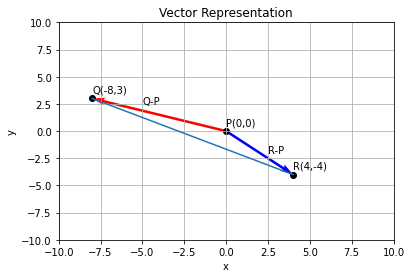
\includegraphics[width=\columnwidth]{solutions/2/2/1/image.png}
\caption{Plot obtained from Python code}
\label{2/2/1/Fig:1}
\end{figure}